\documentclass[border=10pt]{standalone}
\usepackage{mathptmx}
\usepackage{amsmath,bm}
\usepackage{tikz}
\usetikzlibrary{arrows.meta,positioning,fit,calc,backgrounds}
\definecolor{gdark}{HTML}{5E7B5F}
\definecolor{glight}{HTML}{E6E9E4}
\definecolor{gbord}{HTML}{4A634B}
\definecolor{rloss}{HTML}{A8323E}
\definecolor{rsoft}{HTML}{F3DCDD}
\definecolor{note}{HTML}{F4F1E8}
\tikzset{
  dk/.style={draw=gbord,fill=gdark,text=white,rounded corners=3pt,align=center,font=\small,minimum height=12mm,minimum width=30mm,inner sep=5pt},
  lt/.style={draw=gray!60,fill=glight,text=black,rounded corners=3pt,align=center,font=\small,minimum height=12mm,minimum width=30mm,inner sep=5pt},
  ls/.style={draw=rloss,fill=rsoft,text=black,rounded corners=3pt,align=center,font=\small,minimum height=12mm,minimum width=30mm,inner sep=5pt,line width=0.8pt},
  nt/.style={draw=gray!50,fill=note,text=black!80,rounded corners=3pt,align=left,font=\footnotesize,inner sep=6pt},
  ar/.style={-{Stealth[length=2.6mm]},line width=0.8pt,draw=black!75},
  ard/.style={-{Stealth[length=2.6mm]},line width=0.8pt,draw=rloss,dashed},
  lb/.style={font=\footnotesize\itshape,text=black!70,align=center},
  frame/.style={draw=gbord,rounded corners=6pt,dashed,line width=0.7pt,inner sep=8pt},
  ttl/.style={font=\large\bfseries,text=black}
}
\newcommand{\x}{\bm{x}}

\begin{document}
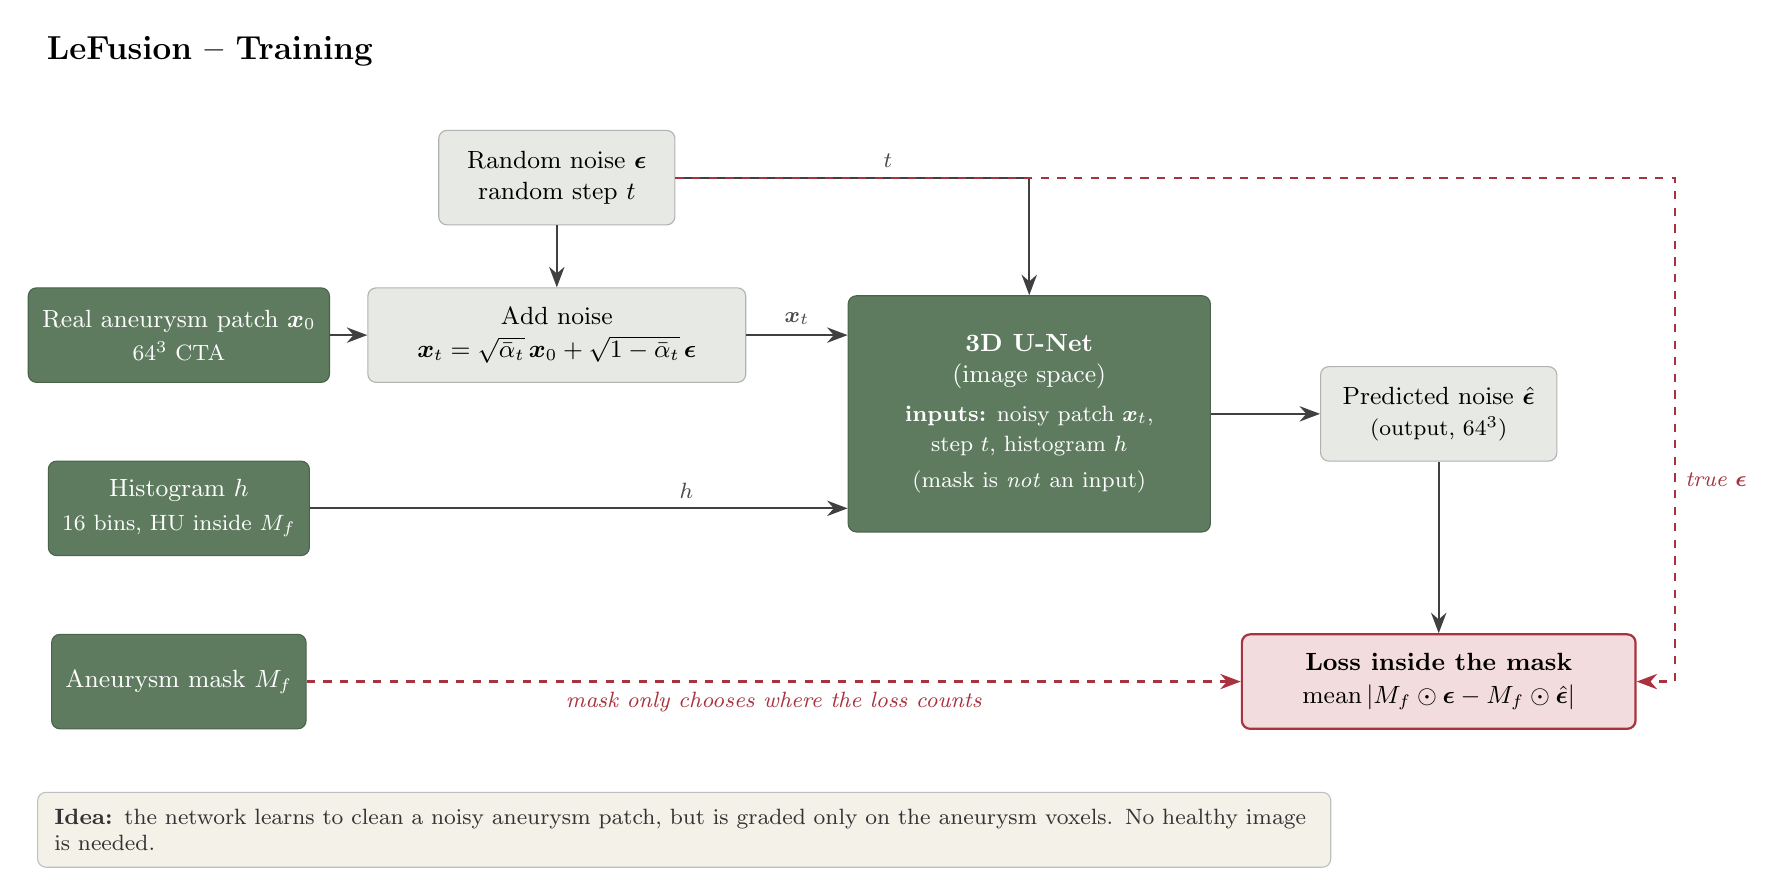
\begin{tikzpicture}[x=1mm,y=1mm]
\node[ttl, anchor=west] at (-18,46) {LeFusion -- Training};
% inputs
\node[dk] (x0) at (0,10) {Real aneurysm patch $\x_0$\\[1pt]\footnotesize $64^3$ CTA};
\node[dk] (h) at (0,-12) {Histogram $h$\\[1pt]\footnotesize 16 bins, HU inside $M_f$};
\node[dk] (mf) at (0,-34) {Aneurysm mask $M_f$};
\node[lt] (eps) at (48,30) {Random noise $\bm\epsilon$\\random step $t$};
\node[lt, minimum width=48mm] (nz) at (48,10) {Add noise\\[1pt]$\x_t=\sqrt{\bar\alpha_t}\,\x_0+\sqrt{1-\bar\alpha_t}\,\bm\epsilon$};
\node[dk, minimum width=46mm, minimum height=30mm] (u) at (108,0) {\textbf{3D U-Net}\\(image space)\\[3pt]\footnotesize \textbf{inputs:} noisy patch $\x_t$,\\\footnotesize step $t$, histogram $h$\\[2pt]\footnotesize (mask is \emph{not} an input)};
\node[lt] (eh) at (160,0) {Predicted noise $\hat{\bm\epsilon}$\\\footnotesize (output, $64^3$)};
\node[ls, minimum width=50mm] (loss) at (160,-34) {\textbf{Loss inside the mask}\\[1pt]$\mathrm{mean}\,|M_f\odot\bm\epsilon-M_f\odot\hat{\bm\epsilon}|$};
\draw[ar] (x0)--(nz); \draw[ar] (eps)--(nz);
\draw[ar] (nz.east) -- node[lb,above]{$\x_t$} (nz.east -| u.west);
\draw[ar] (h.east) -- node[lb,above,pos=0.7]{$h$} (h.east -| u.west);
\draw[ar] (eps.east) -- node[lb,above,pos=0.6]{$t$} (eps.east -| u.north) -- (u.north);
\draw[ar] (u)--(eh); \draw[ar] (eh)--(loss);
\draw[ard] (mf.east) -- node[lb,below,text=rloss]{mask only chooses where the loss counts} (loss.west);
\draw[ard] (eps.east) -- (190,30) |- node[lb,pos=0.3,right,text=rloss]{true $\bm\epsilon$} (loss.east);
\node[nt, text width=160mm, anchor=north west] at (-18,-48) {\textbf{Idea:} the network learns to clean a noisy aneurysm patch, but is graded only on the aneurysm voxels. No healthy image is needed.};
\end{tikzpicture}
\end{document}
